\documentclass[Bachelorarbeit.tex]{subfiles}
\begin{document}
\chapter{Literature Analysis}
The literature analysis began with the topic selection (see chapter \ref{ProblemDescription}). The supervisor told us that the initial chosen topic \textit{Face Detection} is to big to treat within one semester, so the first literature research was done to find a specific topic to handle.\\
The second literature research was done to find information about the chosen topic.
\section{Approach}
All interesting literature which were found and marked as interesting (by scanning the abstract) were saved in a list on the \href{https://ilias.fhv.at/goto.php?target=wiki_298249_Literature_Research_%28LR%29}{Ilias project space}. This articles were read in a more detail afterwards.\\
The structure of the table (see figure \ref{LRT}  make additional sorting (by exporting/copying into an EXCEL) possible and the implementation on ILIAS makes it possible to get access easily to the actual table.

\begin{figure}[!h] %LR table
\centering
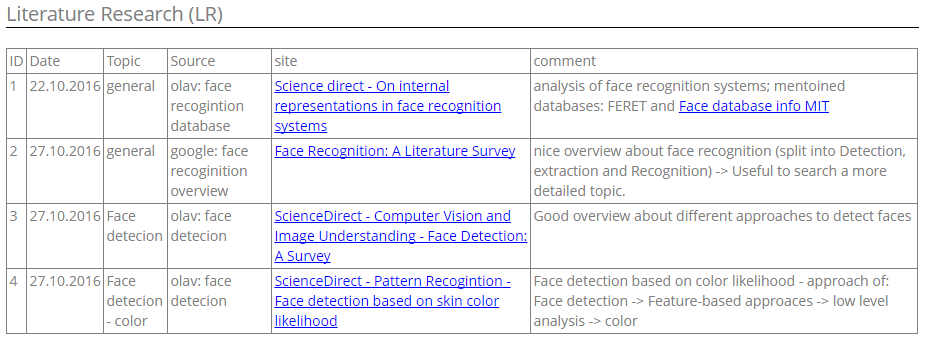
\includegraphics[width=10cm]{./pictures/LR_20161030}
\caption{Literature reasarech table - 30.10.2016. \label{LRT}}
\end{figure}

All literatures which were mentioned in this document are also listed in the bibliography.

\section{LR color based face detection}
%documentation why articles have been selected or rejected. All
%used sources must be mentioned here
\subsection{General Information about Face detection/Face recognition}
The articles in subsections gives an overview of the topic face recognition and face detection. These articles were used to define the chosen topic: "Color based face detection".
\begin{itemize}
\item \textit{Face Detection: A Survey} from \cite{FDASurvey} 
\item \textit{Face Recognition: A Literature Survey} from \cite{FRLiteratureSurvey}    
\end{itemize}

\subsection{Color based face detection}
The article \textit{A Robust Skin Color Based Face Detection Algorithm} from \cite{RobustSkinColorFD} compares the three different color models (RGC, YCbCr and HSI). According to this article the color model YCbCr is widely used in the digital video domain and is more accurate (in detecting faces) than the other to color models. These two arguments are the reason why the color model YCbCr was chosen for this project.\bigskip 

A article which describes step by step how an approach of the color based face detection can be implemented can be found in the article \textit{Face Detection Using Color Thresholding, and Eigenimage Template Matching} from \cite{ColorAndEigenimage}. In this article thresholds for the Cb and Cr are defined.\bigskip 

A different approach to morphological operations can be found in the article \textit{Real Time Detection and Tracking of Human Face using Skin Color Segmentation and Region Properties} from \cite{RTFaceDetection}. This article defines also thresholds for the Cb and Cr.

\end{document}